\section{Classical dynamics}
\label{sec:classical}

\subsection{From regular motion to global chaos}

\Cref{fig:phase_portraits} shows phase portraits for four kick strengths (experiment 01). The orbits start
on the four symmetry lines of the map, $\theta = 0$, $\theta = \pi$, $\theta = p/2$ and
$\theta = p/2 + \pi$. The standard map is a product of two involutions (maps that are their own inverse), and
these lines are their fixed sets, so symmetric periodic orbits and the islands around them cross them. Each
orbit is classified by its finite-time Lyapunov exponent over kicks 2000 to 4000: chaotic if $\lambda > 0.01$.
On a regular orbit displacements grow only linearly, which gives $\lambda \approx \ln 2/2000$, far below the
threshold.

\begin{figure}[!tbp]
  \centering
  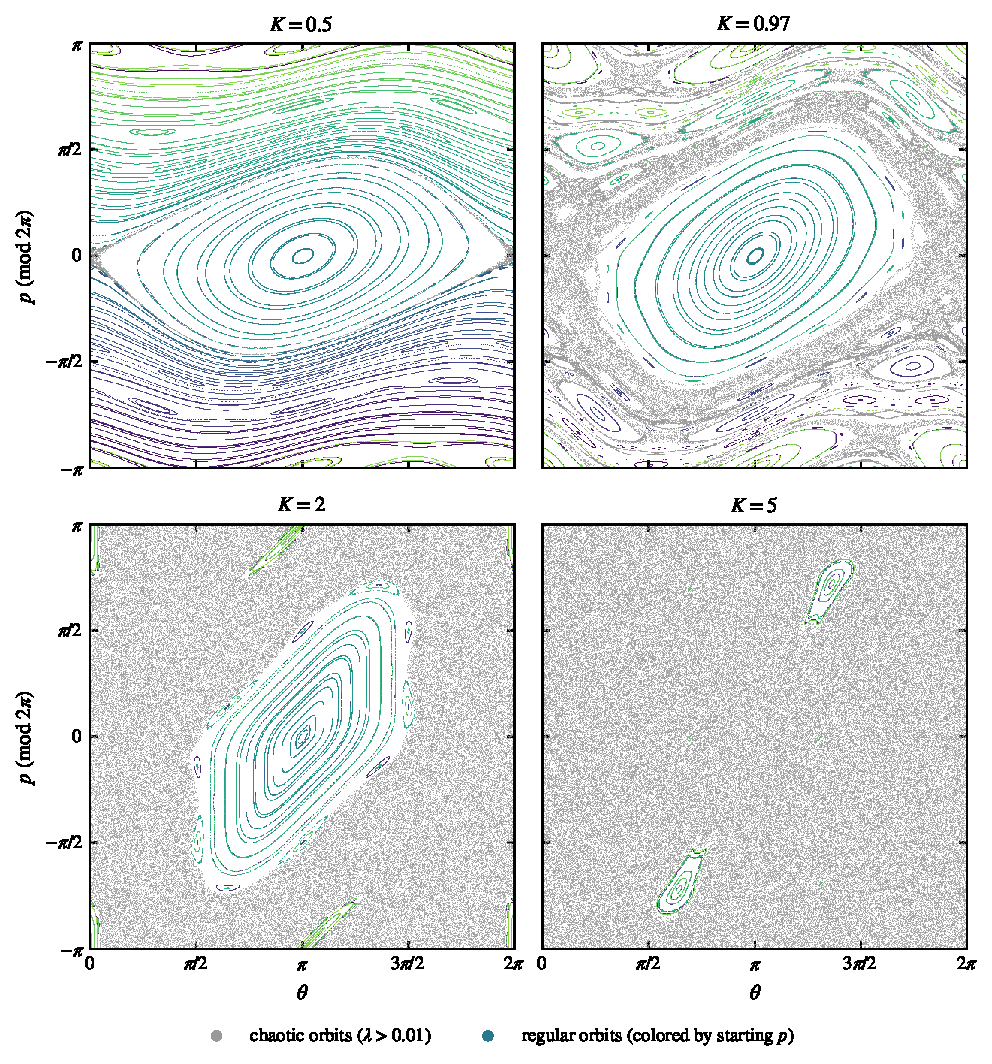
\includegraphics[width=0.78\linewidth]{01_phase_portraits.pdf}
  \caption{Phase portraits of the standard map (experiment 01), with $p$ folded into $[-\pi, \pi)$. Gray:
  chaotic orbits ($\lambda > 0.01$). Colors: regular orbits, colored by their starting momentum. At
  $K = 0.5$ invariant curves span the whole range of $\theta$ and confine the momentum; only a thin chaotic
  layer surrounds the island at $(\pi, 0)$. At $K = 0.97$, just below $K_c = 0.9716$, chaotic layers have
  grown but curves spanning $\theta$ still survive. At $K = 2$ a chaotic sea surrounds the central island,
  and at $K = 5$ almost the whole torus is chaotic, apart from two small islands around a period-2 orbit.}
  \label{fig:phase_portraits}
\end{figure}

\begin{table}[!htbp]
\centering
\small
\begin{tabular}{@{}cccc@{}}
\toprule
$K$ & chaotic area & median $\lambda$ of chaotic orbits & largest $|p_n - p_0|$ in the portrait \\
\midrule
0.5  & 1.2\%  & 0.08 & 2.7 \\
0.97 & 42.6\% & 0.09 & 4.6 \\
2    & 75.5\% & 0.46 & 104 \\
5    & 98.1\% & 0.98 & 628 \\
\bottomrule
\end{tabular}
\caption{Measures of chaos from experiment 01. The chaotic area is the fraction of an $80\times80$ grid of
starting points with $\lambda > 0.01$.}
\label{tab:chaos}
\end{table}

\Cref{tab:chaos} puts numbers on the picture. For weak kicks most orbits are regular, as the
Kolmogorov-Arnold-Moser (KAM) theorem predicts for small perturbations of an integrable system. The
invariant curves that run all the way around in $\theta$ act as walls in momentum: for $K = 0.5$ and 0.97 no
orbit's momentum changes by more than $2\pi$. The last of these curves breaks at
$K_c = 0.971635$, a value Greene found from the stability of periodic orbits that approximate it
\cite{Greene1979}. Above $K_c$ the chaotic layers connect, and a chaotic orbit can wander arbitrarily far in
momentum: at $K = 2$ and 5 the largest momentum changes are 104 and 628 after a few thousand kicks.

Chirikov's resonance-overlap criterion gives a simple estimate of this transition \cite{Chirikov1979}. The
map has resonances at $p = 2\pi n$ with half-width $2\sqrt K$; they overlap when $4\sqrt K \ge 2\pi$, that is,
for $K \ge \pi^2/4 \approx 2.47$. This overestimates the true border by a factor of about 2.5, because
smaller secondary resonances also overlap and destroy the curves earlier, but it captures the mechanism.

The fixed point at $(\theta, p) = (\pi, 0)$ is elliptic for $K < 4$ (its linearized map has trace $2 - K$),
which is why the large central island persists up to $K = 2$. At $K = 5$ it has become unstable, and only
small islands remain, occupying 1.9\% of the torus. For large $K$ the Lyapunov exponent is close to
Chirikov's estimate $\ln(K/2)$ \cite{Chirikov1979}, which comes from averaging $\ln|K\cos\theta|$ over the
chaotic orbit; at $K = 5$ we find $\lambda = 0.98$ against $\ln 2.5 = 0.92$. Chirikov's Table 5.1 lists the
Kolmogorov-Sinai entropy, which for this map equals the mean Lyapunov exponent of the chaotic orbits, divided by
$\ln(K/2)$: 1.20 at $K = 4$ and 1.027 at $K = 6.21$. Our ratio, $0.98/0.92 = 1.07$ at $K = 5$, lies in
between.

\subsection{Diffusion and its Bessel-function corrections}
\label{sec:diffusion}

In the chaotic regime the momentum after $n$ kicks is $p_n = p_0 + K\sum_{j=0}^{n-1}\sin\theta_j$. If the
angles were independent and uniformly distributed, each kick would add $K^2/2$ to the mean square momentum
change, and the motion would be a random walk with the quasilinear diffusion rate
\begin{equation}
  D = \lim_{n\to\infty}\frac{\avg{(p_n - p_0)^2}}{n} = \frac{K^2}{2}.
\end{equation}
Correlations between successive angles change this. With $C_j = \avg{\sin\theta_0\sin\theta_j}$ averaged
over the invariant measure, the exact statement is
\begin{equation}
  D = K^2\Bigl[C_0 + 2\sum_{j\ge1} C_j\Bigr],
  \qquad C_0 = \tfrac12,\quad C_1 = 0,\quad C_2 = -\tfrac12 J_2(K),\quad C_3 = \tfrac12\bigl[J_3^2(K) - J_1^2(K)\bigr],
  \label{eq:D_correlations}
\end{equation}
as derived in \cref{app:correlations}. Keeping lags up to 3 gives the result of Rechester and White
\cite{Rechester1980}, and the first five terms of the later expansion by Rechester, Rosenbluth and White
\cite{Rechester1981} add the leading part of lag 4:
\begin{equation}
  \frac{D}{K^2/2} \approx 1 - 2J_2(K) - 2J_1^2(K) + 2J_3^2(K) + 2J_2^2(K).
  \label{eq:five_term}
\end{equation}
(We have converted their diffusion coefficient, defined with an extra factor $\tfrac12$, to ours.) Since
$J_n(K) \sim \sqrt{2/\pi K}\,\cos(K - n\pi/2 - \pi/4)$ for large $K$, the corrections oscillate with period
$2\pi$ in $K$ and decay like $K^{-1/2}$.

There is one more ingredient. If $K\sin\theta^* = 2\pi l$ for an integer $l$, the point $(\theta^*, p)$
returns to the same angle with its momentum raised by exactly $2\pi l$, so it is a fixed point on the torus
that accelerates forever. It is stable when $|2 + K\cos\theta^*| < 2$, which happens in the windows
$2\pi l \le K \le \sqrt{(2\pi l)^2 + 16}$ \cite{Chirikov1979}, for example $6.28 \le K \le 7.45$ for $l = 1$.
Inside these windows the islands around these \emph{accelerator modes} carry orbits ballistically, and near
them chaotic orbits stick to the islands for long stretches and make long flights. Both effects ruin normal
diffusion, so we keep $K$ away from the windows.

\begin{figure}[!tbp]
  \centering
  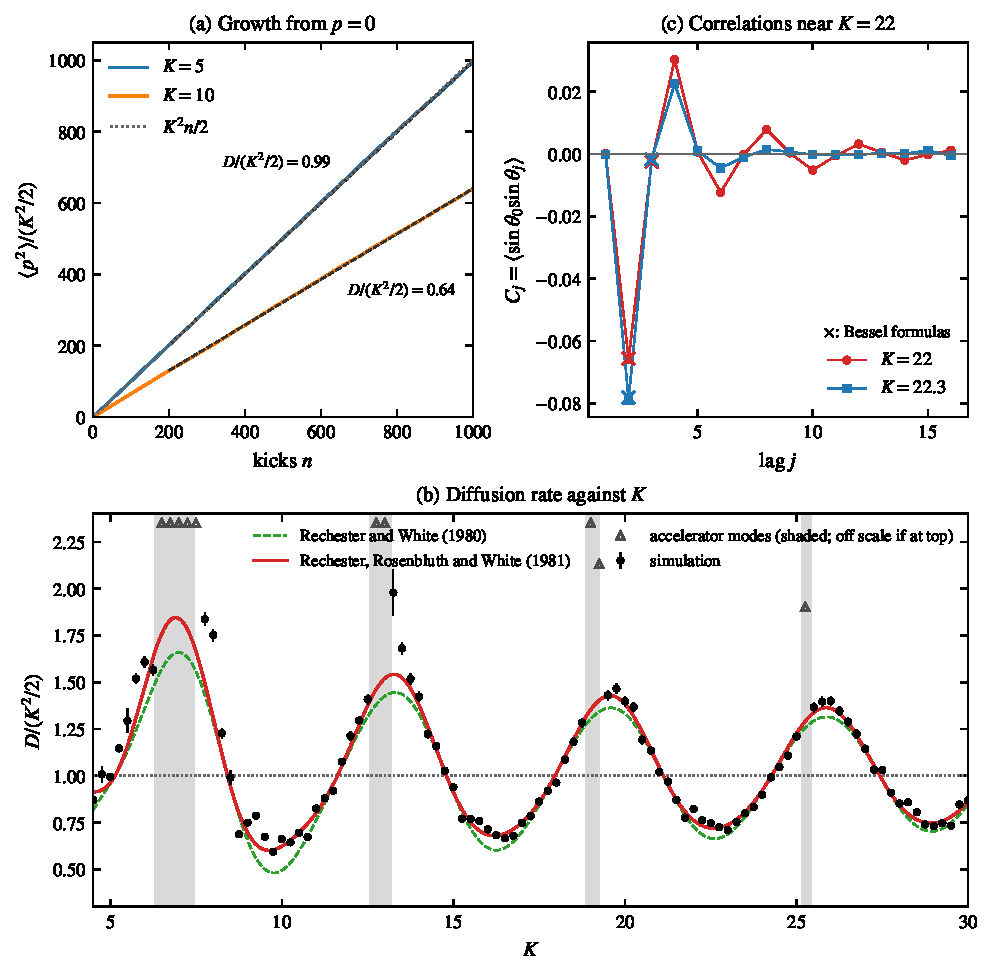
\includegraphics[width=\linewidth]{02_classical_diffusion.pdf}
  \caption{Classical diffusion (experiment 02). (a) $\avg{p^2}/(K^2/2)$ for the ensemble $p_0 = 0$,
  $\theta_0$ uniform (40000 orbits), with the fitted slopes. (b) $D/(K^2/2)$ against $K$ from the torus
  ensemble (10000 orbits per $K$, error bars one standard error), with the four-term formula of
  Rechester and White (dashed), the five-term formula \cref{eq:five_term} (solid), and the accelerator-mode
  windows (shaded; triangles mark values off the scale). (c) The correlations $C_j$ at $K = 22$ and 22.3;
  crosses mark the Bessel-function results for $C_2$ and $C_3$.}
  \label{fig:diffusion}
\end{figure}

\Cref{fig:diffusion} shows the results of experiment 02. Panel (a) confirms linear growth for the
project's ensemble. The slopes give $D/(K^2/2) = 0.995 \pm 0.009$ at $K = 5$ and $0.638 \pm 0.006$ at
$K = 10$, against 0.963 and 0.623 from \cref{eq:five_term}. Panel (b) scans 103 values of $K$ between 4.5 and
30. The measured rate oscillates around the quasilinear value with period about $2\pi$, and away from the
accelerator windows the five-term formula follows it with an rms miss of 0.041. Just outside the windows
the diffusion is strongly enhanced, up to $D/(K^2/2) = 3.2$ at $K = 7.5$.

A few misses are larger than the statistical error allows. In five runs with different random seeds,
$K = 8.75$, 9.25 and 10.75 missed by more than four standard errors every time (by about $-0.11$, $+0.16$
and $-0.06$), and a few other values sat close to that line. Panel (c) shows where such misses come from at
$K = 22$. The measured $C_2 = -0.0658$ and $C_3 = -0.0024$ agree with the Bessel results $-0.0657$ and
$-0.0025$, and the sum up to lag 3 gives 0.728, against 0.727 from the four-term formula. But
$C_4 = +0.030$ adds 0.12 to
$D/(K^2/2)$, and a slowly decaying tail follows, with a sign pattern that repeats every four lags. Summing
the measured correlations up to lag 16 gives 0.823, matching the directly measured 0.821, while the
five-term formula, which contains only the $J_2^2$ part of lag 4, gives 0.762. The truncated formulas are
asymptotic expansions, and they fail wherever the higher correlations happen to be large.

Islands matter for a second reason: they make $D$ depend on the ensemble. At $K = 9.25$ the line $p = 0$
crosses an island that traps about 9\% of the matched ensemble forever. That ensemble gives
$D/(K^2/2) = 0.718$, while the torus ensemble, of which only 0.9\% is trapped, gives 0.800. Both values
are steady over 4000 kicks, so this is not slow convergence. At $K = 4.5$, 5 and every value we tested from
8.75 to 11.25 apart from 9.25, the two ensembles agree to within about two standard errors.
